% Describir el plan de trabajo, las tareas planificadas junto con el tiempo estimiado y el resultado esperado de cada tarea.

\section{Planificación del Trabajo}

La planificación del proyecto se ha descompuesto en paquetes de trabajo, cada uno de estos paquetes incluye una descripción de sus tareas principales junto con su tiempo estimado de desarrollo.

\subsection{Paquetes de Trabajo}

La planificación del proyecto se ha seguido según la planificación que se muestra en la Figura \ref{fig:paquetes}, en donde se muestran los paquetes principales y las tareas asociadas a cada uno.

\begin{figure}[h]
    \centering
    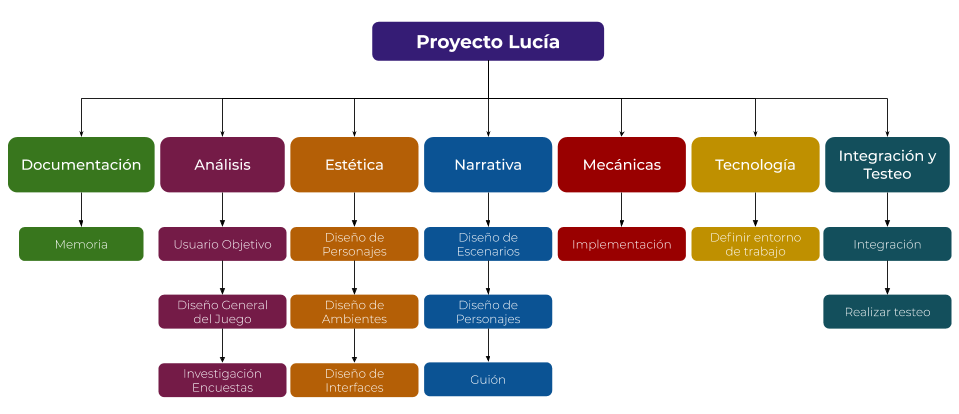
\includegraphics[width=\textwidth]{imgs/paquetes.png}
    \caption{Planificación}
    \label{fig:paquetes}
\end{figure}

\subsection{Descripción de Paquetes}
A continuación presentaremos cada uno de los paquetes de trabajo, con la descripción del paquete, sus tareas principales, los entregables del mismo y una estimación del tiempo necesario para el desarrollo del paquete. Esta información se presentará según la ficha que se muestra en el Cuadro \ref{tab:paquete}.

\begin{table}[h!]
    \centering
    \begin{tabular}{|l|p{10cm}|}
        \hline
        \rowcolor{Gray}
        \textbf{Nombre del Paquete} &  \\
        \hline
        Descripción & \\
        \hline
        Tareas a Realizar & \\
        \hline
        Entregables & \\
        \hline
        Tiempo estimado & \\
        \hline
    \end{tabular}
    \caption{Descripción de los paquetes}
    \label{tab:paquete}
\end{table}

\subsubsection{Documentación}
\begin{table}[h!]
    \centering
    \begin{tabular}{|l|p{10cm}|}
        \hline
        \rowcolor{Green}
        \textcolor{white}{\textbf{Nombre del Paquete}} & \textcolor{white}{\textbf{Documentación}}\\
        \hline
        \rowcolor{Light Green}
        Descripción & Recolección de la información y de las acciones hechas durante el proyecto.\\
        \hline
        \rowcolor{Light Green}
        Tareas a Realizar & Preparación de la Memoria\\
        \hline
        \rowcolor{Light Green}
        Entregables & Memoria del Proyecto\\
        \hline
        \rowcolor{Light Green}
        Tiempo estimado & 5 meses\\
        \hline
    \end{tabular}
    \caption{Paquete de Documentación}
    \label{tab:paquete-documentacion}
\end{table}

\newpage
\subsubsection{Análisis}
\begin{table}[h!]
    \centering
    \begin{tabular}{|l|p{10cm}|}
        \hline
        \rowcolor{Violet}
        \textcolor{white}{\textbf{Nombre del Paquete}} & \textcolor{white}{\textbf{Análisis}}\\
        \hline
        \rowcolor{Light Violet}
        Descripción & Análisis de los requerimientos necesarios para desarrollar el videojuego y la investigación\\
        \hline
        \rowcolor{Light Violet}
        Tareas a Realizar & Usuario Objetivo\\
        \rowcolor{Light Violet}
        & Diseño General del Juego\\
        \rowcolor{Light Violet}
        & Investigación Encuestas\\
        \hline
        \rowcolor{Light Violet}
        Entregables & Documento inicial de diseño\\
        \rowcolor{Light Violet}
        & Encuestas\\
        \hline
        \rowcolor{Light Violet}
        Tiempo estimado & 3 meses\\
        \hline
    \end{tabular}
    \caption{Paquete de Análisis}
    \label{tab:paquete-analisis}
\end{table}

\subsubsection{Estética}
\begin{table}[h!]
    \centering
    \begin{tabular}{|l|p{10cm}|}
        \hline
        \rowcolor{Orange}
        \textcolor{white}{\textbf{Nombre del Paquete}} & \textcolor{white}{\textbf{Estética}}\\
        \hline
        \rowcolor{Light Orange}
        Descripción & Diseño de la gráfica del videojuego\\
        \hline
        \rowcolor{Light Orange}
        Tareas a Realizar & Diseño de Personajes\\
        \rowcolor{Light Orange}
        & Diseño de Ambientes\\
        \rowcolor{Light Orange}
        & Diseño de Interfaces\\
        \hline
        \rowcolor{Light Orange}
        Entregables & Documento de Estética\\
        \rowcolor{Light Orange}
        & Assets Gráficos\\
        \hline
        \rowcolor{Light Orange}
        Tiempo estimado & 2 meses\\
        \hline
    \end{tabular}
    \caption{Paquete de Estética}
    \label{tab:paquete-estetica}
\end{table}

\newpage
\subsubsection{Narrativa}
\begin{table}[h!]
    \centering
    \begin{tabular}{|l|p{10cm}|}
        \hline
        \rowcolor{Blue}
        \textcolor{white}{\textbf{Nombre del Paquete}} & \textcolor{white}{\textbf{Narrativa}}\\
        \hline
        \rowcolor{Light Blue}
        Descripción & Diseño de la narrativa del videojuego\\
        \hline
        \rowcolor{Light Blue}
        Tareas a Realizar & Diseño de Escenarios\\
        \rowcolor{Light Blue}
        & Diseño de Personajes\\
        \rowcolor{Light Blue}
        & Guión\\
        \hline
        \rowcolor{Light Blue}
        Entregables & Documento de Narrativa\\
        \hline
        \rowcolor{Light Blue}
        Tiempo estimado & 1 mes y medio\\
        \hline
    \end{tabular}
    \caption{Paquete de Narrativa}
    \label{tab:paquete-narrativa}
\end{table}

\subsubsection{Mecánicas}
\begin{table}[h!]
    \centering
    \begin{tabular}{|l|p{10cm}|}
        \hline
        \rowcolor{Red}
        \textcolor{white}{\textbf{Nombre del Paquete}} & \textcolor{white}{\textbf{Mecánicas}}\\
        \hline
        \rowcolor{Light Red}
        Descripción & Implementación de las mecánicas diseñadas\\
        \hline
        \rowcolor{Light Red}
        Tareas a Realizar & Implementar mecánicas\\
        \hline
        \rowcolor{Light Red}
        Entregables & Prototipo\\
        \hline
        \rowcolor{Light Red}
        Tiempo estimado & 1 mes y medio\\
        \hline
    \end{tabular}
    \caption{Paquete de Mecánicas}
    \label{tab:paquete-mecanicas}
\end{table}

\newpage
\subsubsection{Tecnología}
\begin{table}[h!]
    \centering
    \begin{tabular}{|l|p{10cm}|}
        \hline
        \rowcolor{Yellow}
        \textcolor{white}{\textbf{Nombre del Paquete}} & \textcolor{white}{\textbf{Tecnología}}\\
        \hline
        \rowcolor{Light Yellow}
        Descripción & Selección de las herramientas a utilizar\\
        \hline
        \rowcolor{Light Yellow}
        Tareas a Realizar & Definir entorno de trabajo\\
        \hline
        \rowcolor{Light Yellow}
        Entregables & \\
        \hline
        \rowcolor{Light Yellow}
        Tiempo estimado & 1 día\\
        \hline
    \end{tabular}
    \caption{Paquete de Tecnología}
    \label{tab:paquete-tecnologia}
\end{table}

\subsubsection{Integración y Testeo}
\begin{table}[h!]
    \centering
    \begin{tabular}{|l|p{10cm}|}
        \hline
        \rowcolor{Aqua}
        \textcolor{white}{\textbf{Nombre del Paquete}} & \textcolor{white}{\textbf{Integración y Testeo}}\\
        \hline
        \rowcolor{Light Aqua}
        Descripción & Integración de todos los elementos del videojuego y la investigación\\
        \hline
        \rowcolor{Light Aqua}
        Tareas a Realizar & Integración\\
        \rowcolor{Light Aqua}
        & Testeo\\
        \hline
        \rowcolor{Light Aqua}
        Entregables & Videojuego final\\
        \hline
        \rowcolor{Light Aqua}
        Tiempo estimado & 2 semanas\\
        \hline
    \end{tabular}
    \caption{Paquete de Integración y Testeo}
    \label{tab:paquete-integracion}
\end{table}

\subsection{Planificación de actividades}
A continuación se mostrará la carta Gantt con la planificación de las actividades y su respectivo tiempo, en base a lo estipulado en los paquetes mencionados.

\begin{sidewaysfigure}
    \centering
    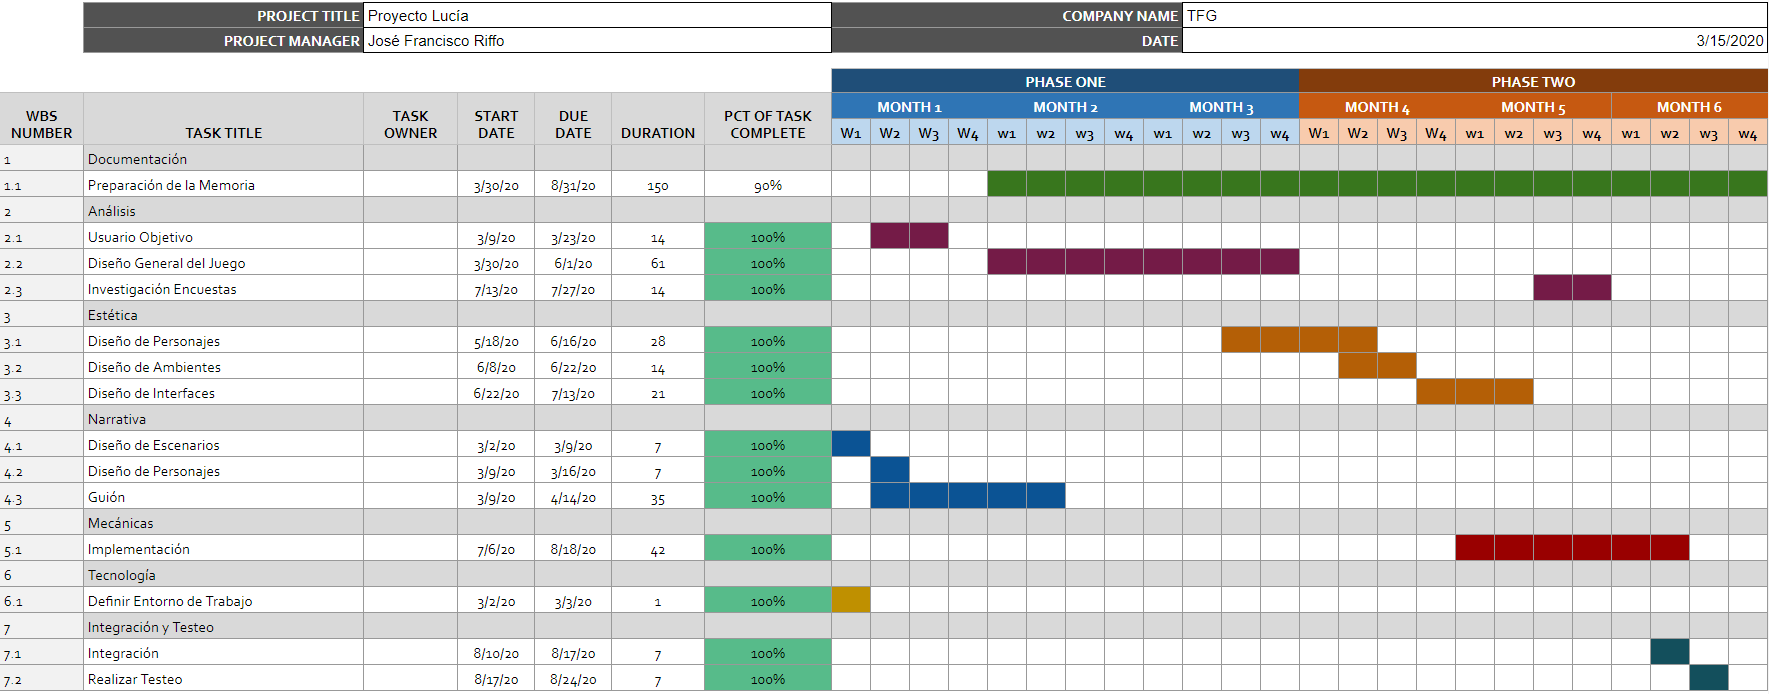
\includegraphics[width=\textwidth]{imgs/gantt.png}
    \caption{Planificación de Actividades}
    \label{fig:gantt}
\end{sidewaysfigure}

\subsection{Metodología de Trabajo}
Dado que para el desarrollo de un videojuego se requiere definir una narrativa, una estética, una mecánica y seleccionar una tecnología, se ha de aplicar una metodología de trabajo que permita trabajar estas componente en paralelo, ya que las decisiones que se tomen en un punto determinado afectan al resto de las componentes.

Debido a la naturaleza del proyecto y la investigación, los paquetes de Narrativa y Análisis son los primeros en ser trabajados, ya que ambos dictaran las bases de como será el resto del proyecto.

Para cada uno de los paquetes de trabajo, se realizarán reuniones periódicas con los tutores del proyecto, quienes supervisarán el trabajo realizado y aplicaran las mejoras y correcciones necesarias.